The blockdiagram of the demodulation is present in figure \ref{fig:blockdiagram}. 
\begin{figure}[h]
 \centering
 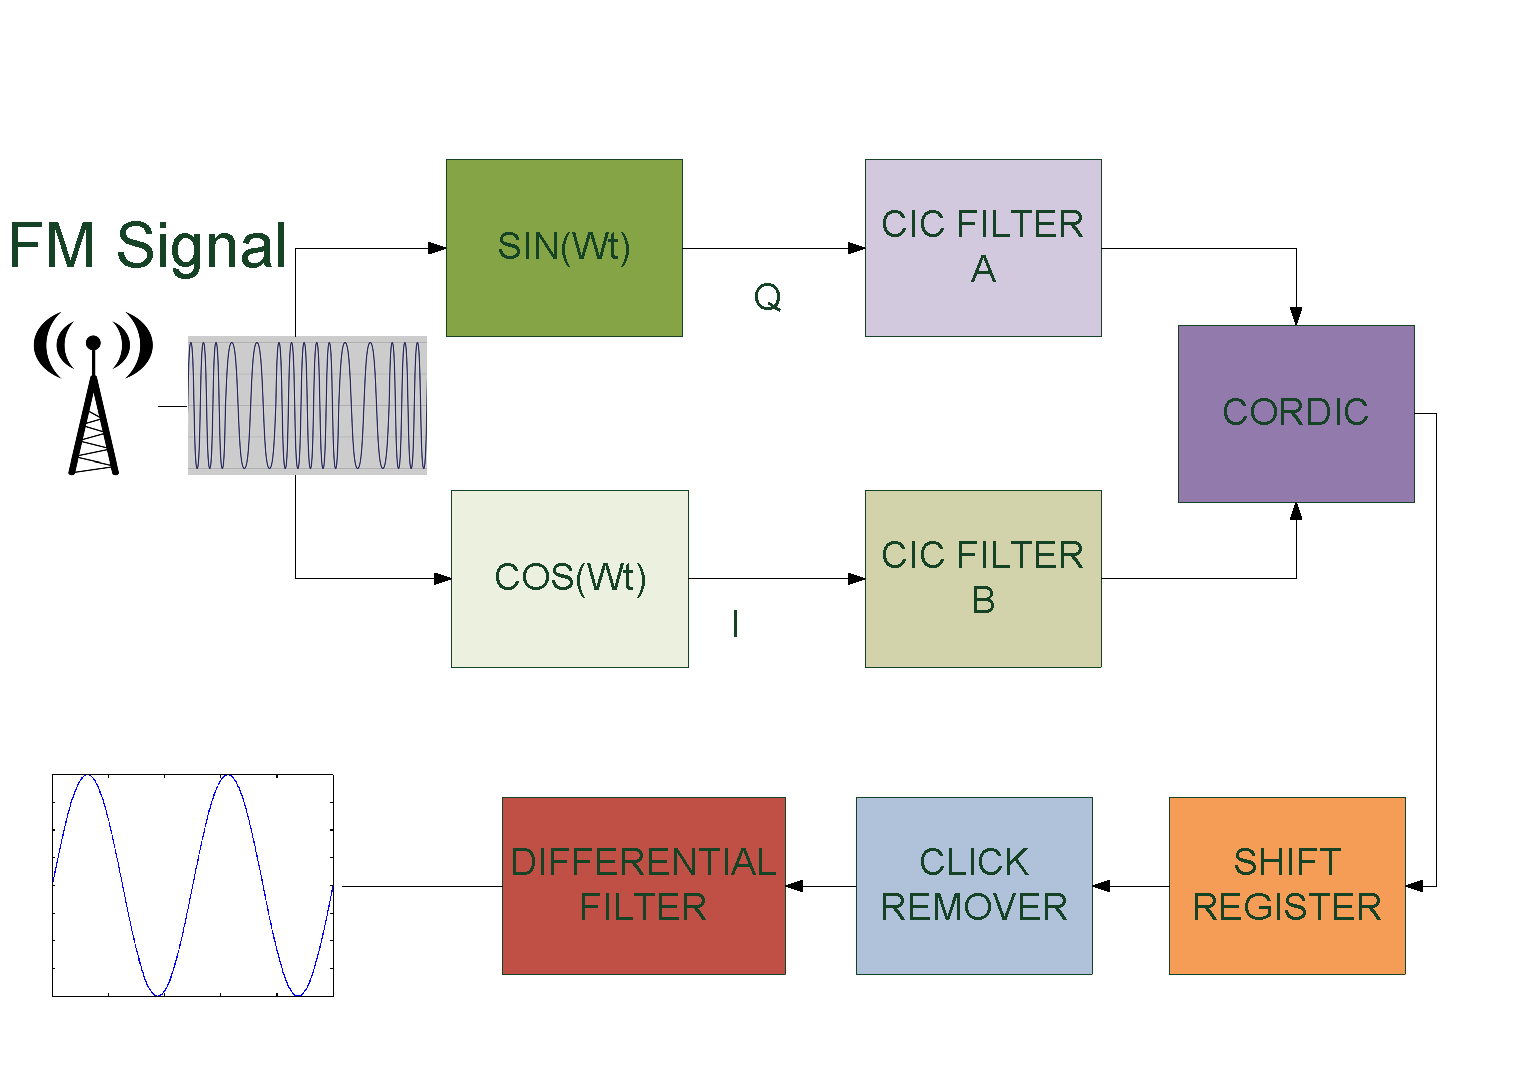
\includegraphics[scale=0.5]{images/blockdiagram.pdf}
 \caption{Blockdiagram of the demodulation}
 \label{fig:blockdiagram}
\end{figure}

The project basically consists of five blocks or modules. These blocks will be described in following sections. To obtain I and Q, it is needed to mix sine and cosine separately to the input signal. Then I and Q will be phase 90 degrees between each other. By mixing cosine it will produces a real in-phase(I) and by mixing sine it produces an imaginary quadrature-phase(Q).